%!TEX root = TQFTbook.tex
%%%%%%%%%%%%%%%%%%%%%%%%%%%%%%%%%%%%%%%%%%%%%%%%%%%%%%%%%%
\chapter{Physical motivation}\label{c:physical-motivation}
In this chapter we provide motivation for the mathematical study of topological
quantum field theories (TQFTs). These theories arise as a special case of more
general quantum field theories (QFTs), so we first look at the physics
definition of QFT. This definition is notoriously non-rigorous, and as of now,
there is no mathematically rigorous definition of QFT in full generality.
Despite this, one can use the non-rigorous physical definition to try to
axiomatize the bare minimum requirements that any sensible QFT should fulfill.

We start with a heuristic introduction to classical and quantum field theories.
Since our purpose is just to motivate the connection to TQFT, we suppress here
many technical details to keep the exposition simple. Interested readers can
find details in numerous textbooks on QFT, such as the physics classic
\cite{peskin-schroeder} or the recent book \cite{etingof-qft},
written for mathematicians.

This chapter is used as motivation only; no results in the remaining
chapters rely on the material of this chapter.


%%%%%%%%%%%%%%
\section{Classical and quantum mechanics}\label{s:mechanics}

In classical mechanics, at any time $t$, a point particle is described by its
position $x(t) \in N$ and its velocity $\dot x(t) \in T_{x(t)}N$. Here $N$ is
the configuration space which, for a point particle, is the same as physical
space, and $T_{x(t)}N$ is the tangent space to $N$ at the point $x(t)$.
(For a more general mechanical system, $N$ can be some other space of
configurations.)
The trajectory of a particle is a map from the
time interval $[t_0,t_1]$ to $N$:
\begin{equation}
	\ga\colon[t_0,t_1] \rightarrow N. \nonumber
\end{equation}
We are using the position variable $x$ and the trajectory $\ga$
interchangeably. They are both continuous maps from the time interval to the
configuration space, but the notation $\ga$ is better suited for quantum
mechanics where we will be considering all such maps.

The equations of motion are usually derived using the Lagrangian formalism.
Namely, for each trajectory $\ga(t)$ we define its action:
\begin{equation}
	S[\ga]= \int_{t_0}^{t_1} L(x(t),\dot x(t))\, dt \nonumber
\end{equation}
where $L(x, \dot x)$ is a smooth function on $TN$ called the Lagrangian.
The precise form of
the Lagrangian function $L$ depends on the physics governing the motion of the
particle.

The least action principle (more appropriately called the stationary action
principle) states that the actual trajectory that the physical particle takes
is one for which the functional variation of the action vanishes (in the class
of all trajectories with fixed starting and ending positions):
\begin{equation}\label{e:stationary-path}
	\delta S[x_{\mathrm{ph}}] = 0, \qquad x_{\mathrm{ph}}(t_0) = x_0,\quad x_{\mathrm{ph}}(t_1) = x_1.
\end{equation}
This condition leads to the so-called Euler--Lagrange equations, which are the
equations of motion in classical mechanics.


In quantum mechanics, the state of the particle is described by the wave
function $\psi$, a vector in some Hilbert space $\calH_N$; for a single
particle moving in the configuration space $N$, $\calH_N$ is the space of
square-integrable functions on $N$:
\begin{equation*}
	\psi \in \calH_N \cong L^2(N).
\end{equation*}

The evolution of a quantum-mechanical system from time $t_0$
to $t_1$ is described by the evolution operator:
\begin{equation*}
	U_{t_0,t_1}\colon \calH_N \to\calH_N.
\end{equation*}

Traditionally, this operator is defined using the Schr\"odinger equation.
However, there is an alternative approach, based on Feynman's path integral.
Namely, let us express the evolution operator using an integral kernel:
\begin{equation}
	(U_{t_0,t_1} \psi)(x_1) = \int_{N} K(x_1,x_0) \psi(x_0) dx_0
\end{equation}

The Feynman path integral prescription states that this integral
kernel can be written as:
\begin{equation}\label{e:feynman1}
	K(x_1,x_0) = \int_{\substack{\ga(t_0)=x_0 \\
  \ga(t_1)=x_1}} e^{ \frac{i}{\hbar} S[\ga] } D\ga
\end{equation}
where $\hbar$ is the reduced Planck constant.

The physical essence of this formula is that all possible paths taking the
particle from $x_0$ at $t_0$ to $x_1$ at $t_1$ contribute to its evolution.
This prescription of integration over all trajectories is sometimes called
``sum over histories''.

Formula \eqref{e:feynman1} expresses the evolution operator in terms of
an integral over the infinite-dimensional space of paths. Making sense of such
integrals is non-trivial; however, heuristically one can argue that in the
limit $\hbar \to 0$, the integral in \eqref{e:feynman1} is dominated by the
contributions from neighborhoods of the critical points of the action. For
finite-dimensional integrals of this form, the method of stationary phase allows
one to write an asymptotic expansion in powers of $\hbar$; using that as
inspiration, one can also write similar formulas for the asymptotic expansion of
the integral \eqref{e:feynman1}. The lowest-order term in this expansion
corresponds to the contribution from the classical path defined in
\eqref{e:stationary-path}.

In Table~\ref{tab:mechanics}, we summarize the main structures of classical
mechanics and the analogous quantities in quantum mechanics. In the next
section, we will use this prescription of sum over histories to define time
evolution in a quantum field theory.

\begin{table}[ht]
  \centering
  \begin{tabular}{|r|l|l|}
  	 \hline
    &\textbf{Classical mechanics} & \textbf{Quantum mechanics} \\[5pt]
    \hline
    Position
    &$x\in N$ (configuration space)
    & $\psi \in \calH_N \cong L^2(N)$ \\[5pt]
    Trajectory
    &$\gamma\colon [t_0, t_1]\to N$
    &$U_{t_0,t_1}\colon \calH_N\to \calH_N$ \\[5pt]
    Action
      &\multicolumn{2}{c|} {$S[\gamma]=\int L(\gamma,\dot\ga) dt$}
      %& $K(x_1,x_0) = \int e^{\frac{i}{\hbar} S[\gamma]} D\ga$
      \\[5pt]
    Laws of motion
    &\parbox[t]{5cm}{Stationary action principle\par
    	\quad $\delta S[\ga]=0$ (fixed endpoints)
    }
    & \parbox[t]{5.5cm}{
    	Sum over histories \par
    	$(U\psi)(x_1) = \int_N K(x_1, x_0) \psi(x_0) dx_0$\par
       $K(x_1,x_0) = \int e^{\frac{i}{\hbar} S[\gamma]} D\ga$
    }
      \\
    \hline
  \end{tabular}
\medskip
  \caption{Summary of the main structures in classical and quantum mechanics}
  \label{tab:mechanics}
\end{table}


%%%%%%%%%%%%%%
\section{Classical and quantum field theory}\label{s:field-theory}
Let us now move from mechanics to field theory. In field theory,
the position variable $x\in N$ is replaced by a field $\ph$,
which is typically either a function on $N$ (with values in some target space
$V$), a section of a vector bundle, or a connection. For simplicity, let us
assume that the field $\ph$ (at a given time) takes values in $V$:
\begin{equation*}
	\ph\colon N \rightarrow V.
\end{equation*}
As is common in the physics literature, we will assume that the field $\ph$
is smooth enough for all purposes. We denote by $\calF_N$ the space of all
fields (at a fixed moment of time); in the simplest example above,
$\calF_N=C^\infty (N,V)$. This space is the analog of the configuration space
$N$ in classical mechanics.

The analog of a trajectory is now a field $\ph(x,t)$ on spacetime $M = N
\times [t_0,t_1]$. If the space $N$ is $(n-1)$-dimensional, then
spacetime $M$ is $n$-dimensional; the corresponding field theory is referred
to as an $n$-dimensional field theory.


 Note that the space $N$ plays a different role here than in mechanics. In
 a field theory, $N$ is the domain of the field $\ph$, whereas in mechanics, the
 configuration space $N$ was the target of the ``position field'' $x$. From this
 perspective, we can think of the discussion in the previous section as a
 $(0+1)$-dimensional field theory of the position field $x\colon \text{point}
 \to N$.

As in mechanics, equations of motion come from the stationary action principle.
Namely, for a field $\ph$ defined on spacetime $M=N\times[t_0, t_1]$, we define
the action functional by
\begin{equation}
	S[\ph] = \int_{t_0}^{t_1} L(\ph, \del_{\mu} \ph) dt = \int_{t_0}^{t_1} \left(
	\int_N \calL(\ph, \del_{\mu} \ph) d^{n-1} x \right) dt
\end{equation}
Here $\calL$ is called the Lagrangian density; it depends on the value of the
field $\ph$ at the point $(x,t)$, its first derivatives $\del_\mu \ph$, and the
metric $g$ on spacetime.

The classical equations of motion again follow from the stationary action
principle: $\delta S[\ph]=0$. This is equivalent to a system of PDEs on
$\ph$, called the \emph{Euler--Lagrange equations}.
%\begin{equation}
%	\del_{\mu} \left( \frac{\del \calL}{\del (\del_{\mu} \ph)} \right) -
%\frac{\del \calL}{\del \ph} = 0
%\end{equation}

%This easily generalizes to a Lagrangian that depends on more than one field.
%The equations coming from $\delta S[\ph]=0$ are generally called the
%Euler-Lagrange equations of motion.

Similar to how we moved from classical to quantum mechanics, it is natural to
expect that in quantum field theory, the state of the system is described by a
functional $\psi \in \calH_N = L^2(\calF_N)$. The space $\calF_N$ is
infinite-dimensional, and there is no canonical Lebesgue measure that we can
define for it, so the exact meaning of $L^2$ is unclear; for the
moment, let us ignore that.


The time evolution operator $U_{t_0,t_1}\colon \calH_N \rightarrow \calH_N$
can again be defined using the path integral.
Given a state $\psi$ at time $t_0$, the final state $U\psi$ at time $t_1$
can be written as:
\begin{equation}\label{e:time-evolution}
  \begin{aligned}
	(U \psi)[\ph_1] &= \int_{\calF_N} K(\ph_1,\ph_0) \psi[\ph_0] D \ph_0\\
	K(\ph_1,\ph_0) &= \int_{\substack{\Phi|_{t_0}
  =\ph_0 \\ \Phi|_{t_1}=\ph_1}} e^{\frac{i}{\hbar} S[\Phi]} D\Phi.
  \end{aligned}
\end{equation}
Here $\Phi=\Phi(x,t)$ is a field on spacetime $M=N\times[t_0,t_1]$ with given
values at $t=t_0$, $t=t_1$; it is the analog of the path $\ga$ in mechanics, and
$D\Phi$ is some (not yet defined) measure on the space of fields.


Note that the integral in \eqref{e:time-evolution} does not explicitly use the
decomposition of spacetime $M$ as a product of space $N$ and time interval
$[t_0, t_1]$: it only uses the metric on $M$ (which is used in the Lagrangian
density) and the fact that $M$ has two boundary components, $N_0=N\times\{t_0\}$
and $N_1 = N\times \{t_1\}$. The same integral makes perfect sense if we allow
spacetime $M$ to have a different topology: for any $n$-dimensional manifold $M$
whose boundary is presented as $\del M=\ov{N_0}\sqcup N_1$ (where the bar
denotes orientation reversal), formula \eqref{e:time-evolution} defines an
operator $U\colon \calH_{N_0}\to \calH_{N_1}$.



The above formulas freely use integrals over infinite-dimensional spaces of
paths/fields, which are very hard to define rigorously; there are many
continuum quantum field theories for which a complete rigorous construction of
the path integral is not currently available. Usually the best one can do is to
write the asymptotic formulas, expanding the operator $U$ or the kernel $K$ as
a series in powers of $\hbar$, and even that requires a lot of work.

However, if we are willing to ignore these problems for now, we can
use the path integral formula \eqref{e:time-evolution} to establish various
properties of QFT. For example,
it is easy to show the composition property
\begin{equation*}
U_{t_0,t_2}= U_{t_1,t_2} U_{t_0,t_1}.
\end{equation*}
Indeed, since a field $\Phi\in \calF_{N\times [t_0,t_2]}$ is the same as a
pair of fields $\Phi_1\in \calF_{N\times [t_0,t_1]}$,
$\Phi_2\in \calF_{N\times [t_1,t_2]}$ whose values at the common boundary
$N\times\{t_1\}$ coincide, and $S[\Phi]=S[\Phi_1]+S[\Phi_2]$,  we get
\begin{equation}\label{e:gluing}
  K_M(\ph_2,\ph_0) = \int_{\calF_N}
  K_{M_2}( \ph_2,\ph_1) K_{M_1}(\ph_1, \ph_0) D \ph_1
\end{equation}
where $M=N\times [t_0,t_2]$, $M_1=N\times [t_0,t_1]$, and
$M_2=N\times [t_1,t_2]$.


More generally, the same (non-rigorous) argument shows that for an arbitrary
spacetime $M$, we can cut $M$ along a codimension-one submanifold $N$ and split
the path integral into integrals over the two resulting pieces, which share $N$
as a common boundary.



In the next section, we will try to bypass these rigor-related problems by
approaching QFT in a more axiomatic manner. The main structures appearing
in classical and quantum field theories are summarized in
Table~\ref{tab:qft}.

\begin{table}[h]
	\centering
	\begin{tabular}{|r|l|l|}
		\hline
		&\textbf{Classical field theory} & \textbf{QFT} \\[5pt]
		\hline
		Field/State &$\ph \in \calF_N$
		& $\psi \in \calH_N \cong L^2(\calF_N)$ \\[5pt]
		Trajectory
		&$\ph\in \calF_{M}$, $M=N\times[t_0, t_1]$
		&$U_{t_0,t_1}\colon \calH_N\to \calH_N$ \\[5pt]
		Action
		& \multicolumn{2}{c|}{$S[\ph]=\int_M \calL(\ph, \del_\mu\ph) d^{n}x$}
		%&$K(\ph_1,\ph_0) = \int e^{\frac{i}{\hbar} S[\Phi]} D\Phi$
    \\[5pt]
		Laws of motion
		&\parbox[t]{5cm}{Euler--Lagrange equations\par
			\quad $\delta S[\ph]=0$
		}
		& \parbox[t]{6cm}{
			$(U \psi)[\ph_1] = \int_{\calF_N} K(\ph_1,\ph_0) \psi[\ph_0] D \ph_0$\par
      $K(\ph_1,\ph_0) = \int e^{\frac{i}{\hbar} S[\Phi]} D\Phi$
		}\\
		\hline
	\end{tabular}
	\caption{A schematic comparison of main structures in classical
    and quantum field theory. See main text for details.}
	\label{tab:qft}
\end{table}

%%%%%%%%%%%%%%%%%%%%%%%%%%%
\section{Axioms of quantum field theory}\label{s:axioms-field-theory}

Let us ignore the problems involved in the above definition of QFT and
only focus on the formal properties that any sensible quantum field theory
should satisfy, in particular on a few
axioms that are necessary for the transition to TQFTs.

Taking motivation from the path integral formulation of QFT outlined in the
previous section, we define a QFT as consisting of the following data:
\begin{itemize}
  \item For every closed $(n-1)$-dimensional manifold $N$, we have a
    \emph{Hilbert space} $\calH_N$.
  \item For every $n$-dimensional manifold $M$ together with a decomposition
    $\del M=\ov{N_0}\sqcup N_1$, we have the evolution operator $Z_M\colon
   \calH_{N_0}\to \calH_{N_1}$, given by the path integral formula
   \eqref{e:time-evolution}. (Previously, we used $U$ for the time
  evolution; we switch the notation to $Z$, which is more common in QFT.)
\end{itemize}

These two pieces of data should satisfy certain conditions for consistency:

\begin{enumerate}
  	\item {\bf Disjoint union axiom}: Assume that $N$ is disconnected:
      $N=N_1\sqcup N_2$. Then for the space of fields, we have
      $\calF_{N}=\calF_{N_1}\times \calF_{N_2}$. Using the heuristic definition
      $\calH_N=L^2(\calF_N)$, we therefore require
    \begin{equation}\label{e:qft-axiom1a}
      \calH_{N_1\sqcup N_2} \cong \calH_{N_1}\otimes \calH_{N_2}.
    \end{equation}
  
    Similarly, for a disjoint union of two $n$-manifolds with boundary, we 
    require
    \begin{equation}\label{e:qft-axiom1b}
      Z_{M_1\sqcup M_2} = Z_{M_1}\otimes Z_{M_2}.
    \end{equation}



  \item {\bf Gluing axiom}: The evolution operators defined in this way satisfy
    the gluing axiom, which is a generalization of \eqref{e:gluing}.

    Consider a manifold $M$ that can be cut into two manifolds $M_1$ and $M_2$
    along a codimension-one submanifold $N$; see \firef{f:gluing} for an
    illustration. If $\partial M = \overline{N_0} \sqcup N_1$, then
    $\del M_{1} = \overline{N_0} \sqcup N$, and
    $\del M_{2} = \overline{N} \sqcup N_1$.

    The gluing axiom says that the operator $Z_{M}$ is the composition of the
    operators $Z_{M_1}$ and $Z_{M_2}$:
    \begin{equation}\label{e:gluing-axiom}
    	Z_{M} = Z_{M_2} \circ Z_{M_1}.
    \end{equation}
	In the path integral picture, this is a natural expectation. Instead of
	computing the path integral over the entire manifold $M$, we can compute it
	in two (or more) steps. Evolving a state $\psi$ from $\calH_{N_0}$ to
	$\calH_{N}$ with the operator $Z_{M_1}$, and then evolving the state
	$Z_{M_1} \psi$ from $\calH_{N}$ to $\calH_{N_1}$ with the operator
	$Z_{M_2}$, produces the state $(Z_{M_2} \circ Z_{M_1}) \psi$. We expect this
	final state to equal $Z_M \psi$ for every initial state $\psi$.

      Note that the manifolds do not need to be cylinders. If we consider the
      case where $M_1=N\times [t_0,t_1]$, $M_2=N\times [t_1,t_2]$, then we
      recover \eqref{e:gluing} from the previous section.
    \begin{figure}[ht]
    	\centering

    	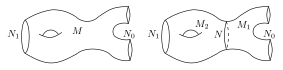
\includegraphics{figures/c1-fig01.svg}

    	\caption{Cutting a manifold $M$ into two manifolds $M_1$ and $M_2$ along
      a codimension-one submanifold $N$. The gluing axiom asserts that
      $Z_M=Z_{M_2} \circ Z_{M_1}$.}
    	\label{f:gluing}
    \end{figure}

    The gluing axiom is a very strong axiom. It allows us to compute the path
    integral of a manifold from smaller pieces. The gluing axiom tells us how
    the (path integrals of) smaller pieces are to be glued along their
    boundaries in order to reconstruct the path integral of the original
    manifold. The underlying assumption that we can compute the path integrals
    of smaller pieces individually makes the locality of the theory manifest.
\end{enumerate}


Note that for the empty space $\varnothing$, the space of fields on
$\varnothing$ is a 1-point set, so $L^2(\calF_\varnothing)=\C$; thus, it is
natural to expect $\calH_\varnothing=\C$. This is also compatible with the
disjoint union axiom, since $\varnothing$ is the unit of the disjoint union
operation: $\calH_{N} \cong \calH_{N \sqcup \varnothing} \cong \calH_{N}\otimes
\calH_{\varnothing}$. Thus, for a closed spacetime (i.e., $\del M=\varnothing$),
we get an operator
\begin{equation}
	Z_M\colon \C\to \C.
\end{equation}
In other words, $Z_M\in \C$ is a number; in physics it is usually called the
\emph{partition function}\index{partition function} and denoted by $Z(M)$.

%%%%%%%%%%%%%%%%%%%%%%%%%%%%%%%%%%%%%%%%
\section{Topological QFT}\label{s:tqft}

So far we have not specified what we mean by ``manifold''. Usually in physics
the spacetime is an oriented pseudo-Riemannian manifold, with a metric of
signature $(1, n-1)$. However, we will be interested in a very special case,
namely when all the structures above do not use the metric on spacetime; thus,
we only require $M$ to be an oriented smooth manifold. Such theories are called
\emph{topological}. The most famous example of such a theory is Chern--Simons
theory\footnote{This is a minor simplification: Chern--Simons theory is not 
  strictly topological -- it has framing anomaly. We will discuss it in 
  more detail in \chref{c:321}} (see \cite{witten-jones}), in which the 
spacetime $M$ must be
3-dimensional, and fields are $\SU(r)$ connections on $M$. After choosing a
trivialization of the bundle, these fields can be described by one-forms,
usually denoted by $A$, with values in the Lie algebra $\su(r)$. The action is
then given by
\begin{equation}
  S[A] = \frac{k}{4 \pi} \int_M \tr(A\wedge dA + \tfrac{2}{3}A\wedge A\wedge A).
\end{equation}

The ``level'' $k$ is a fixed integer parameter of the theory. Although the
numerical value of the Chern--Simons action may change by an integer multiple of
$2\pi k$ under a change of trivialization, the exponentiated action $e^{i S[A]}$
is unchanged. The important thing to note here is that the path integrals
defined using this action do not depend on the choice of the metric. So the
partition functions assigned by this QFT are invariant under
orientation-preserving diffeomorphisms. (It turns out that there are other
observables in this theory besides the partition functions, namely the Wilson
loops, but our preliminary definition of a TQFT does not take these observables
into account.) We can axiomatize the invariance under diffeomorphisms as a
defining property of a topological theory. Together with the axioms of a QFT, we
get the following preliminary definition:

\begin{predefinition}\label{d:ptqft}
  An $n$-dimensional topological quantum field theory (TQFT) is the following
  collection of data:
  \begin{itemize}
    \item For every closed $(n-1)$-dimensional oriented smooth manifold $N$, a
      vector space $Z_N$
    \item For every compact $n$-dimensional oriented manifold $M$ with boundary
      $\del M=\ov{N_0}\sqcup N_1$, a linear operator
      $Z_M\colon Z_{N_0}\to Z_{N_1}$,
  \end{itemize}

  such that

  \begin{itemize}
  	\item Orientation-preserving diffeomorphisms preserve this data
  	\item This data satisfies the disjoint union axiom and the gluing axiom
  	  defined above.
  \end{itemize}

\end{predefinition}

There is a lot more detail to be filled in, but that requires some preparation.
We will provide a more precise definition, due to Atiyah \cite{atiyah}, later
(see \deref{d:tqft}).

Remarkably, topological theories are much easier to define rigorously than
general QFTs. For example, as we show later, in a TQFT all vector spaces
assigned to $(n-1)$-dimensional manifolds are automatically finite-dimensional,
thus avoiding all analytical difficulties with convergence. And instead of
defining a TQFT by a path integral or other global construction (which can be
very hard to do), we can try to construct TQFTs by defining $Z(M)$ for
``elementary blocks'' and gluing every manifold from them. For example, for
$n=2$, any compact oriented surface can be obtained by gluing copies of the
disk, the cylinder, and the pair of pants.
\begin{center}
  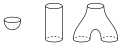
\includegraphics{figures/c1-fig02.svg}
\end{center}

Of course, we need to have some compatibility conditions to ensure that
different ways of gluing the manifold from pieces give the same result;
essentially, we are trying to define manifolds by ``generators and
relations''. For $n=2$ it is not too hard (we will do so in
\chref{c:2d-classification}); for larger $n$, it is harder --- e.g., for
$n=3$ we can consider the so-called Heegaard decompositions (which already
requires infinitely many blocks, namely all handlebodies of arbitrary
genus) or use surgery along (framed) links. The difficulty lies in how fast the data
grows with higher dimensions. Ideally, we would want the number of
generators/relations to be as small as possible in a TQFT, or at least
finite. This leads to the notion of an extended TQFT.

%%%%%%%%%%%%%%%%%%%%%%%%%%%%%%%%%%%%%%%%%%
\section{Toward extended TQFT}\label{s:xtqft}
So far we have talked about cutting a manifold into smaller manifolds with
boundaries. By assigning appropriate data to manifolds with boundaries, we
could glue them back and assign a topological invariant to all possible closed
$n$-manifolds. But why stop at manifolds with boundary? If we allow manifolds
with corners of any codimension, the set of ``elementary blocks'' is greatly
simplified: any manifold can be glued together from just one kind of local
block, namely an $n$-simplex. Such theories are called fully extended (or
sometimes local) TQFTs; see \cite{lurie-cobordism}.

But the price we pay is algebraic complexity. In our discussion so far, a TQFT
assigned a number to a closed $n$-manifold, and a vector space to a
codimension-one manifold. If we also allow cutting along codimension-2
manifolds, what kind of data should be assigned to them? And then what about the
next level?


One possible approach to describing  TQFTs with pieces of any codimensions
is by using the language of higher categories. Very informally, an
$n$-category is an algebraic structure which has objects, 1-morphisms
between them, 2-morphisms between 1-morphisms, and so on, up to
$n$-morphisms. Defining it rigorously quite difficult (we will talk more
about higher categories in \chref{c:higher-cat}). Thus, we could try to
assign to a every zero-dimensional manifold an object of $n$-category, to a
1-dimensional object, a 1-morphism, and so on. This leads to the notion of
\emph{extended TQFT}.


This chapter was roughly centered around the theme that the subject of TQFT
aims to sidestep the analytical difficulties associated with QFTs. One could,
however, also argue for the viewpoint that the mathematical study of TQFTs is
actually a step in dealing with analytical difficulties that the current
formulation of QFT suffers from. In either case, we hope the reader is
convinced that the subject of TQFT lies at a very interesting intersection of
modern physics and mathematics.


